
%Schriftgröße, Layout, Papierformat, Art des Dokumentes
\documentclass[12pt,oneside,a4paper]{scrreprt}

%Einstellungen der Seitenränder
\usepackage[left=3cm,right=3cm,top=2cm,bottom=2cm,includeheadfoot]{geometry}

%neue Rechtschreibung
%\usepackage{ngerman}

%Umlaute ermöglichen
\usepackage[utf8]{inputenc}
\usepackage{graphicx}

\usepackage{xspace}
\usepackage{paralist}
\usepackage{float}

\usepackage{_style/xml}

\usepackage{chngcntr}
\counterwithout{figure}{chapter}

%Kopf- und Fußzeile
\usepackage{fancyhdr}
\pagestyle{fancy}
\fancyhf{}

\fancyhead[L]{\mypackagename}
\fancyhead[R]{\myauthor}
%Linie oben
\renewcommand{\headrulewidth}{0.5pt}

%Linie unten
\renewcommand{\footrulewidth}{0.5pt}

\newcommand{\mypackagename}{StochasticPetriNets\xspace}

\newcommand{\myauthor}{Andreas Rogge-Solti}
\newcommand{\mytitle}{\mypackagename}
\newcommand{\mysubtitle}{Stochastic Petri net package.\\~ \\
Can be used to enrich existing Petri net models with stochastical information obtained from a log.\\~ \\
Allows different parametric and non-parametric models to specify probabilistic timing of transitions.
}


\graphicspath{{.}{./img/}}

% allows for clickable comments, references, etc. in pdf
\usepackage[pdftex]{hyperref}
\hypersetup{
	pdftitle={\mytitle},           % title
    pdfauthor={\myauthor}, % author
    pdfcreator={\myauthor}, % creator of pdf
    unicode=true,          % non-latin characters in bookmarks?
    pdffitwindow=false,    % window fit to page when opened
    pdfstartview={FitH},   % fits width of the page to the window
    pdftoolbar=true,       % show acrobat toolbar?
    pdfmenubar=true,       % show acrobat menu?
    colorlinks=false,      % false: boxed links; true: color links
    linkcolor=black,       % color of internal links
    urlcolor=black,        % color of external links
    citecolor=black,       % color of links to bibliography
    filecolor=black       % color of file links
}

\begin{document}
\begin{titlepage}
\author{\myauthor} 
\title{\mytitle} 
\subtitle{\mysubtitle}
\date{\today} 
\maketitle
\end{titlepage}

\chapter*{\mypackagename}

\subsection*{Packages}

\subsubsection{Requires:}
\begin{compactitem}
  \item PetriNets
  \item TransitionSystems
  \item PNetReplayer
  \item PNetAlignmentAnalysis
  \item Widgets
\end{compactitem}

\subsubsection{Required By:}
\begin{compactitem}
  \item RepairLog
\end{compactitem}

\subsection*{Contained Plugins}

\subsubsection{Importing / Exporting stochastic Petri Nets}
\begin{compactitem}
  \item PNML export: (stochastic) PNML files
  \item PNML import: PNML Stochastic Petri Net files
\end{compactitem}

\subsubsection{Enriching Petri nets with stochastic information}
\begin{compactitem}
  \item Enrich Petri net with performance data
  \item Enrich Petri net with performance data (default mapping)
\end{compactitem}

\subsubsection{Remaining time Prediction \& Experiments}
\begin{compactitem}
  \item Predict duration by Simulation (Single case)
  \item Predict durations (real experiment)
  \item Predict duration by Simulation (Simulated experiment)
\end{compactitem}

\subsection*{License}
\begin{compactitem}
  \item LGPL as-is
  \item GPL when used in combination with R (for log-spline density estimation)
\end{compactitem} 


\section*{Introduction}
\label{sec:intro}
Stochastic Petri nets can be used to model performance aspects of a Petri net.
\begin{itemize}
  \item What ratio of cases follows the upper path in my model?
  \item How long does it take to finish activity \emph{A}?
  \item How long will my current case take?
\end{itemize}
These and further analysis questions can not be answered by pure Petri nets. Therefore different ways to encorporate stochastic execution information into Petri nets were devised. See \cite{ciardo1994characterization} for an overview about different expressivity and analysis capabilities of stochastic Petri net formalisms that were proposed in literature.

In this plugin, we assume stochastic Petri nets to not be restricted to any special parametric form of duration distributions, i.e., we use simply \emph{SPN} in the convention of \cite{ciardo1994characterization}.

\subsubsection{Semantics}
For the execution semantics, we stick to the text-book semantics defined for GSPNs in~\cite{marsan1984class}. However, we allow generalized distributions, and do not restrict times to be exponentially distributed. We use the \emph{race semantics with enabling memory}\footnote{If you're interested, see the original discussion of different execution semantics in~\cite{marsan1989execution}.}, as initially defined in \cite{marsan1989execution}. This semantics allows to model time-outs in a process model, as well as parallelism. The same semantics is also used in the popular analysis tool TimeNET \cite{german1995timenet}. 

Transitions are separated into immediate transitions (firing without taking time) and timed transitions (delayed by a random duration) 
\begin{compactitem}
  \item a priority $p$ (used to specify sets of transitions that always fire before those with lower priority, $p$ is 0 for timed transitions, $p > 0$ for immediate transitions)
  \item a weight (used to probabilistically choose a transition from the group of highest priority transitions)
  \item a duration distribution (capturing the random delay of firing for timed transitions) 
\end{compactitem}

The semantics is as follows:
\begin{compactitem}
  \item determine the set of transitions $t_{enabled}$ that are candidates for being enabled (all transitions that have $> 1$ input tokens on their input places)
  \item determine the highest priority $p$ of these transitions.
  \item remove all transitions from $t_{enabled}$ with a lower priority than $p$
  \begin{compactitem}
    \item if $p > 0$, we choose an immediate transition randomly based on their weights.
    \item if $p = 0$,  the timed transitions race for the right to fire. Each pick a random duration from their distribution (sample a random value).
  \end{compactitem}
\end{compactitem}




 
\chapter*{Installation}
\label{chap:installation}
\begin{figure}[H]
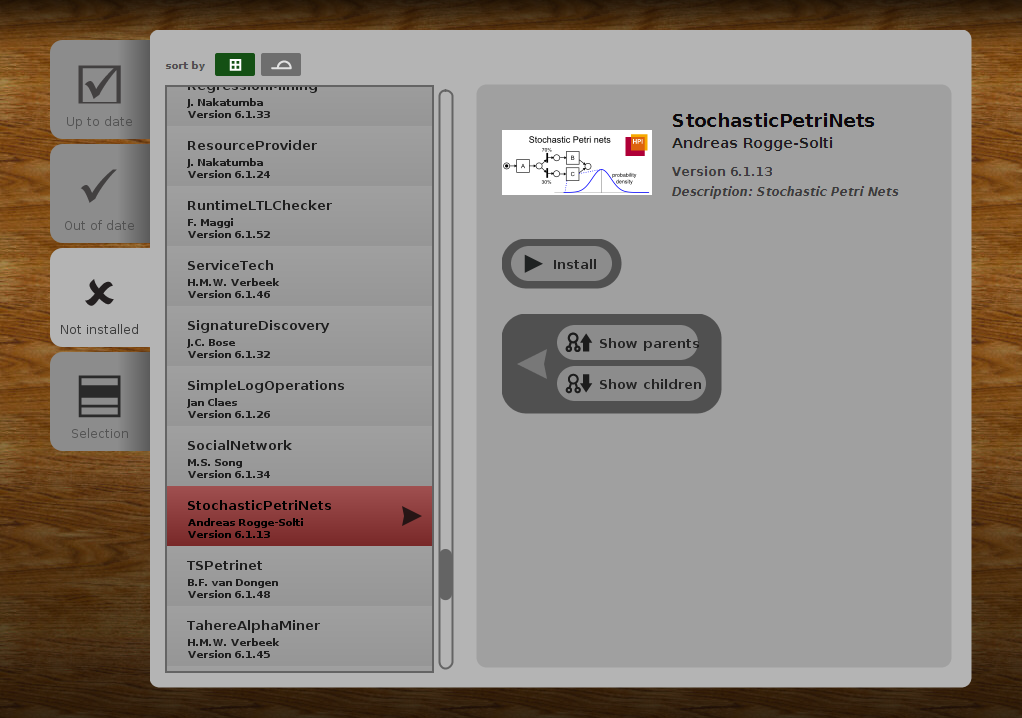
\includegraphics[width=\textwidth]{installer.png}
\caption{Select \& install the StochasticPetriNet Package.}
\label{fig:installation}
\end{figure}


\subsubsection*{About}
The StochasticPetriNet package contains plugins to import and export stochastic Petri nets in the Petri net markup \texttt{.pnml} format.
It allows to convert aligned Logs / Petri net models, i.e., Manifests (output of the \emph{PNetReplayer}-plugin), to stochastic Petri nets.
A visualizer is included. And a prediction experiment comparing predicted times from Transition system based prediction and Petri net based predictions of remaining process durations.

\pagebreak
\section*{Optional: Install R for log spline density estimations}
\label{sec:optional} 
If you want to try the Log-spline density estimator, you need to install the R-project. \url{http://www.r-project.org/}
It is based on the CRAN \texttt{logspline} package by Charles Koopenberg \url{http://cran.r-project.org/web/packages/logspline/index.html}

Proceed with the following steps:
\begin{itemize}
  \item Download and install R \url{http://www.r-project.org/}
  \item startup R and run \texttt{ install.packages("logspline")}
  \item install the binaries for the Java-to-R bridge \texttt{ install.packages("rJava")}
  \item the \mypackagename package needs to point java to the native JRI library, that was installed with rJava. Make sure to add the VM-argument:\\
  -Djava.library.path=\ldots~ points to that binary. 
  \item make sure your environment variable \texttt{R\_HOME} points to your R installation containing the binaries (for linux, this might be \texttt{/usr/lib/R}, or \texttt{/usr/lib64/R})
\end{itemize}

\subsubsection{Note:}
The license of the plug-in will be \textbf{GPL}, if you use it with R and the logspline package.

\pagebreak
\chapter*{Usage}

\begin{figure}[H]
\centering
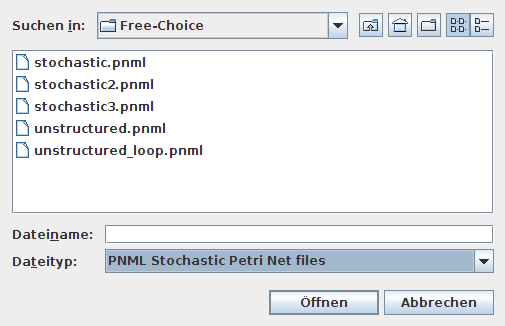
\includegraphics[width=0.6\textwidth]{import.png}
\caption{Importing stochastic Petri nets stored in .pnml-format}
\label{fig:import_dialog}
\end{figure}

\section*{Load an existing annotated PNML file}
You can just click on the import\ldots~button on the top right corner of the ProM workbench and select a \texttt{.pnml} file with a stochastic Petri net, cf. Fig.~\ref{fig:import_dialog}.
The stochastic extension is added as a \texttt{<toolspecific>} annotation to each transition. An example \emph{immediate} transition could look like this:

\lstset{language=XML}
\begin{lstlisting}
    <transition id="tr4">
        <name>
          <text>t_start</text>
        </name>
        <graphics>
          <position x="59" y="92" />
          <dimension x="10" y="32" />
        </graphics>
	<toolspecific tool="StochasticPetriNet" version="0.1">
	  <property key="priority">1</property>
	  <property key="weight">1</property>
      	  <property key="distributionType">IMMEDIATE</property>
          <property key="distributionParameters"></property>
        </toolspecific>
      </transition>
\end{lstlisting}
Note that the \texttt{tool}-attribute needs to be set to \texttt{"StochasticPetriNet"}
 
The annotated properties for transitions are:
\begin{itemize}
  \item the \emph{priority} of the transition. Semantics: of all enabled transitions, only the transitions with highest priority may fire. Immediate transitions have \emph{priority} $\geq$ 1, whereas timed transitions have \emph{priority} = 0.  
  \item the \emph{weight} of the transition. Used for probabilistic choice between two or more immediate transitions. Each transition will be used proportionally often as their weight is in relation to the whole weight of all enabled transitions.
  \item the \emph{distributionType} is used to specify which parametric/non-parametric type the timed transition has, or if it is an \texttt{IMMEDIATE} transition. For timed transitions, following distribution types are supported:
  \begin{itemize}
    \item BETA
    \item EXPONENTIAL
    \item NORMAL
    \item LOGNORMAL
    \item GAMMA
    \item UNIFORM
    \item WEIBULL
    \item GAUSSIAN\_KERNEL
    \item HISTOGRAM
    \item LOG\_SPLINE (optional, only powered with R-support) 
  \end{itemize}
  \item the \emph{distributionParameters} contains a semicolon \texttt{;} separated list of double values. The number of parameters depends on the type of the distribution. For example, the \texttt{NORMAL} distribution needs two parameters: $\mu$ mean, and $\sigma$ standard deviation.
  The \texttt{EXPONENTIAL} distribution only needs one parameter: $\lambda$ the firing rate.
  Nonparametric methods like the gaussian kernel density estimator store all sample values separated by a semicolon.
\end{itemize}

\section*{Enrich Petri net by manual replay using \emph{Replay PN for Performance analysis}}
If no stochastically enriched \texttt{.pnml}-file exists yet, you can enrich an existing petri net with performance data gathered from a log. 
Therefore, replay the log in the model for performance analysis (PNetReplayer plugin) and obtain \emph{Manifest}
Use the \emph{Manifest} as input to the plugin \texttt{Enrich Petri net with performance data}

\subsection*{Prerequisites}
\begin{compactitem}
  \item load a Log file with timestamp attributes.
  \item a fitting Petri net model that can be mapped to the log file.
  (try either mining algorithms, or model it yourself with e.g. Yasper, or CPNTools.)  
\end{compactitem} 

\begin{figure}[H]
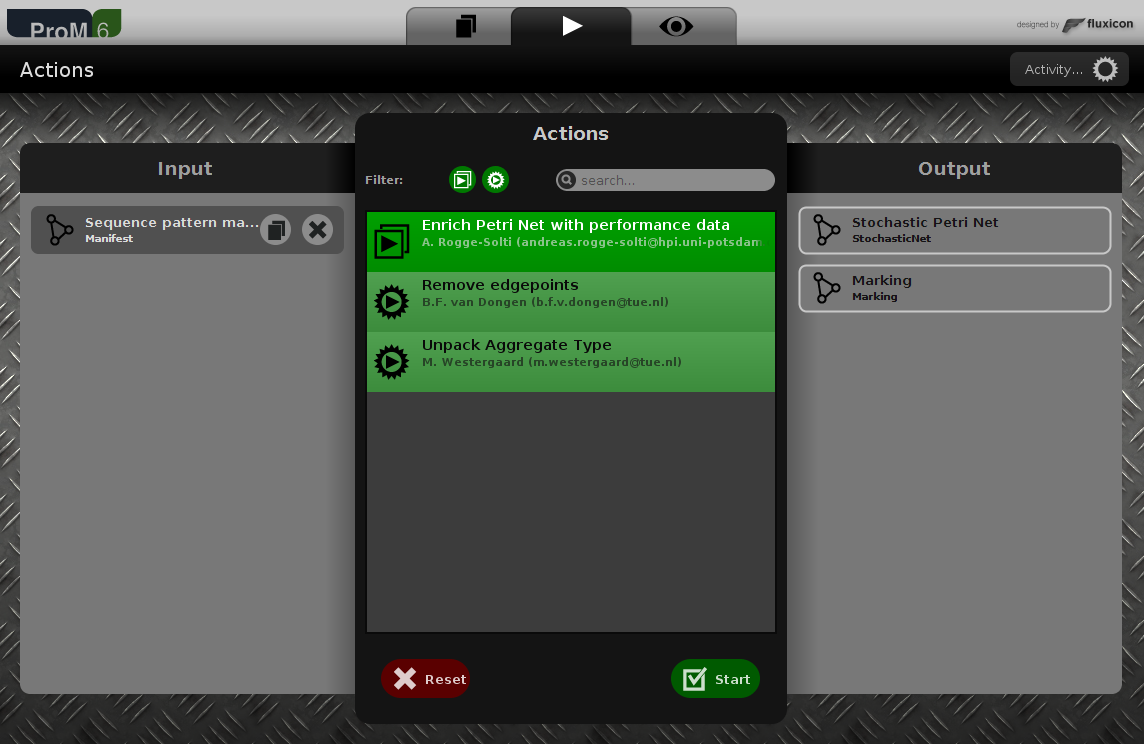
\includegraphics[width=\textwidth]{enrich2_1.png}
\caption{Convert a replayed Log and Petri net (Manifest) to a StochasticNet}
\label{fig:convert_manifest}
\end{figure}

\subsection*{Type of distributions}
Select the kind of distributions that shall be used in the stochastic Petri net: (Fig.~\ref{fig:distribution_type_selection})
\begin{figure}[h]
\centering
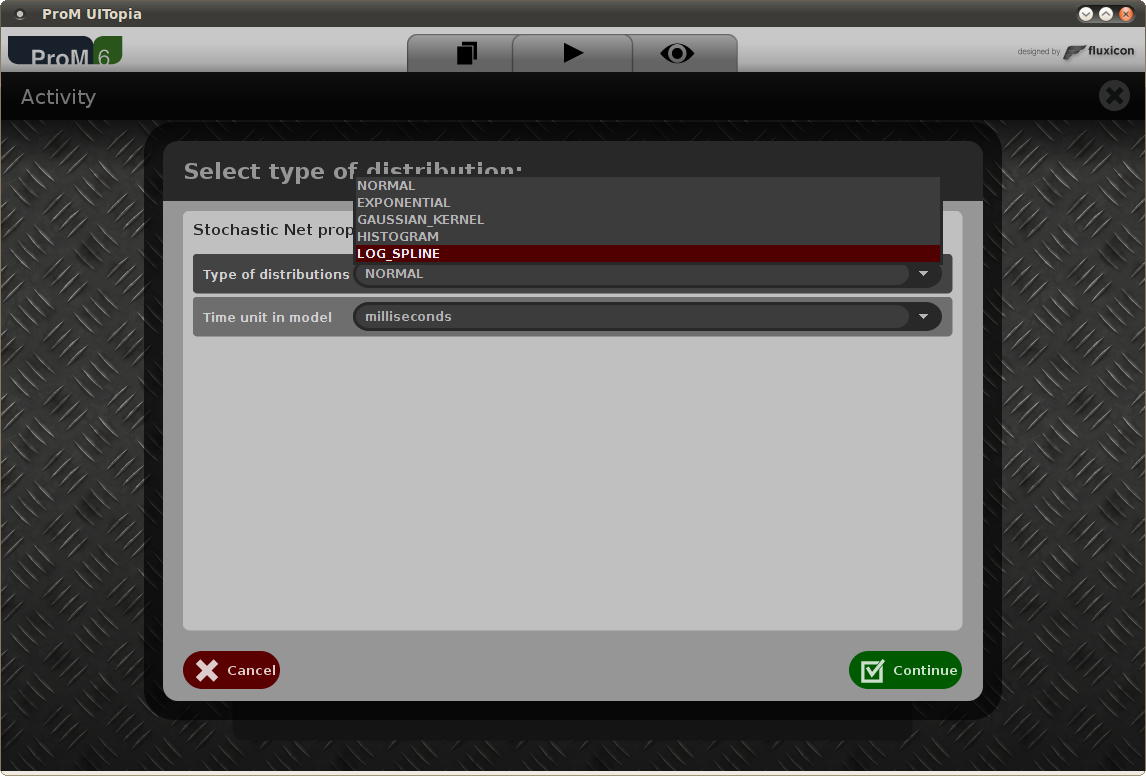
\includegraphics[width=0.85\textwidth]{enrich1_2.png}
\caption{Select the type of the distributions at timed transitions}
\label{fig:distribution_type_selection}
\end{figure}

\begin{compactitem}
  \item The \texttt{NORMAL} type assumes normally distributed transition durations, and collects means and standard deviations of the historical activity durations.
  \item The \texttt{EXPONENTIAL} type assumes exponetially distributed delays for transition durations and uses the observed sample means as parameter for exponential activity durations.
  \item The \texttt{GAUSSIAN\_KERNEL} type performs a kernel density fit with Gaussian kernels, cf. Fig.~\ref{fig:gauss_kernel}
  \item The \texttt{HISTOGRAM} type creates simple histograms for visualization.
  \item The \texttt{LOG\_SPLINE} type is only available, if you installed \texttt{R} correctly, cf. Sect.~\ref{sec:Installation}
\end{compactitem} 

\subsection*{Time unit in model}
You can select the unit of the parametric models. This unit will influence also the bin-size of the \texttt{HISTOGRAM} distribution type.

\section*{Enrich Petri net by automatic replay using default mapping by name}
If your Petri net model that you want to enrich corresponds to the log, such that the transition names are equal, and each visible transition has corresponding events, you can save yourself the wizard of the \emph{Replay Petri net for performance analysis} plugin and use Log and Petri net model directly as input to the \emph{Enrich Petri net with performance data (default mapping)} plugin.


\section*{Visualize the stochastic Petri net}
Once you have loaded a stochastic Petri net successfully, or you managed to enrich a Petri net with performance data from a Log,
you can view it. Open the \emph{Stochastic Petri Net Visualizer}, as shown in Fig.~\ref{fig:open_visualizer}

\begin{figure}[H]
\centering
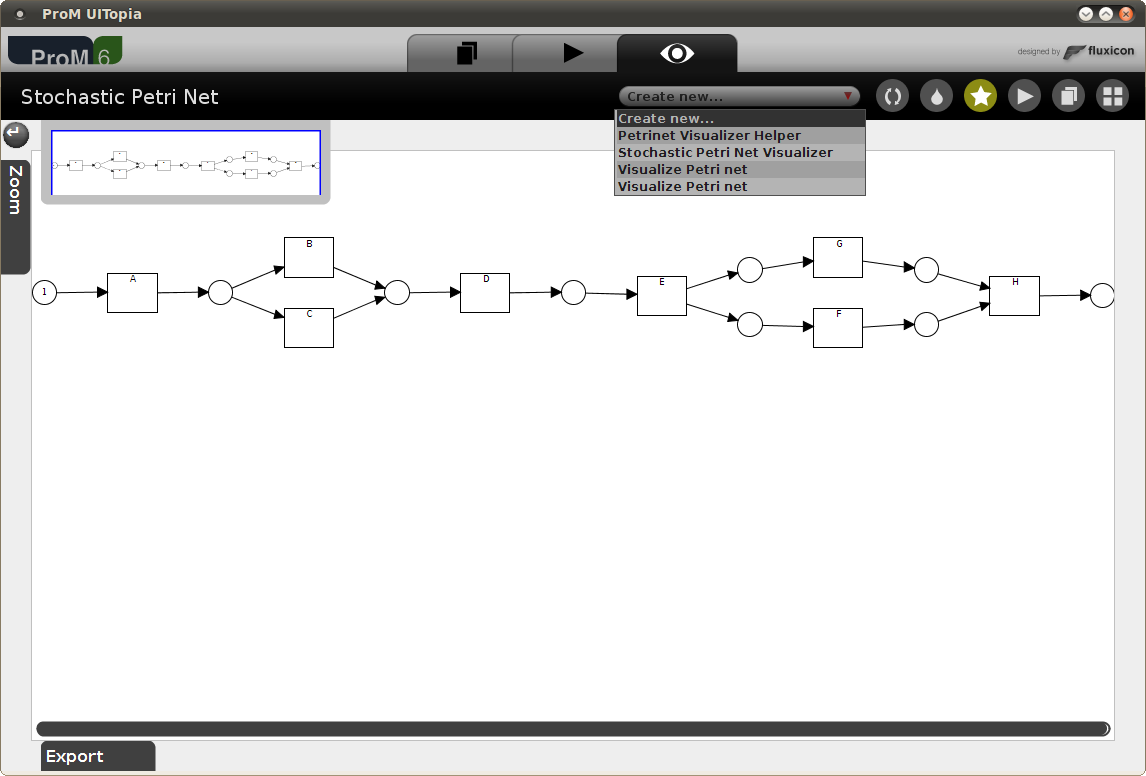
\includegraphics[width=0.95\textwidth]{visualize.png}
\caption{Select the \texttt{Stochastic Petri Net Visualizer} to see the stochastic annotations.}
\label{fig:open_visualizer}
\end{figure}

\begin{figure}[H]
\centering
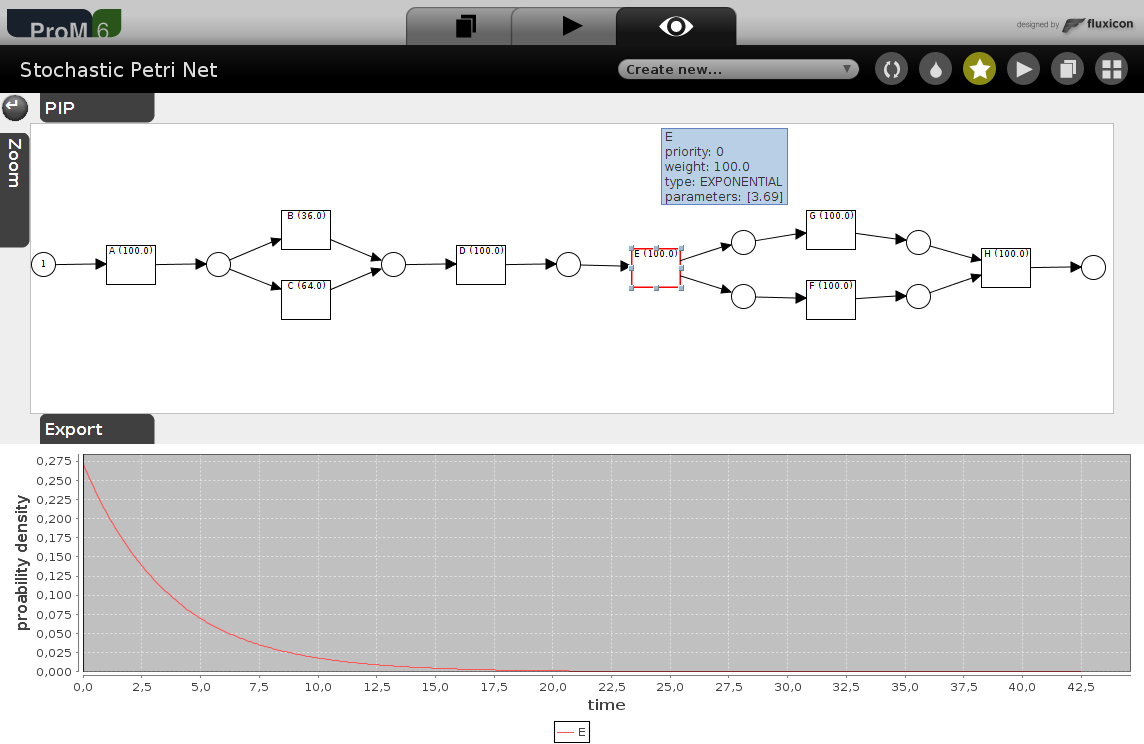
\includegraphics[width=0.95\textwidth]{visualize2.png}
\caption{Exponential distributions -- fit to the observed mean durations.}
\label{fig:exponential_distributions}
\end{figure}

\begin{figure}[H]
\centering
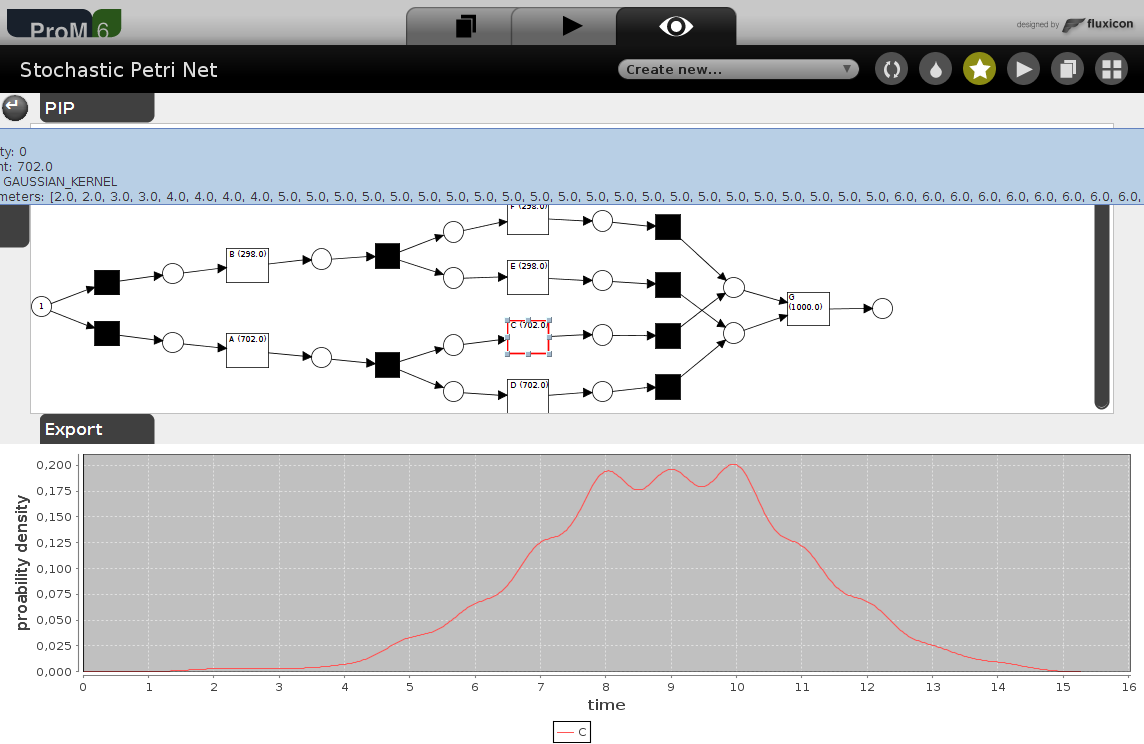
\includegraphics[width=0.95\textwidth]{visualize2_gaussian_kernel.png}
\caption{Activity duration densities obtained from the observed data. Fit by kernel density regression with Gaussian kernels.}
\label{fig:gauss_kernel}
\end{figure}

\begin{figure}[H]
\centering
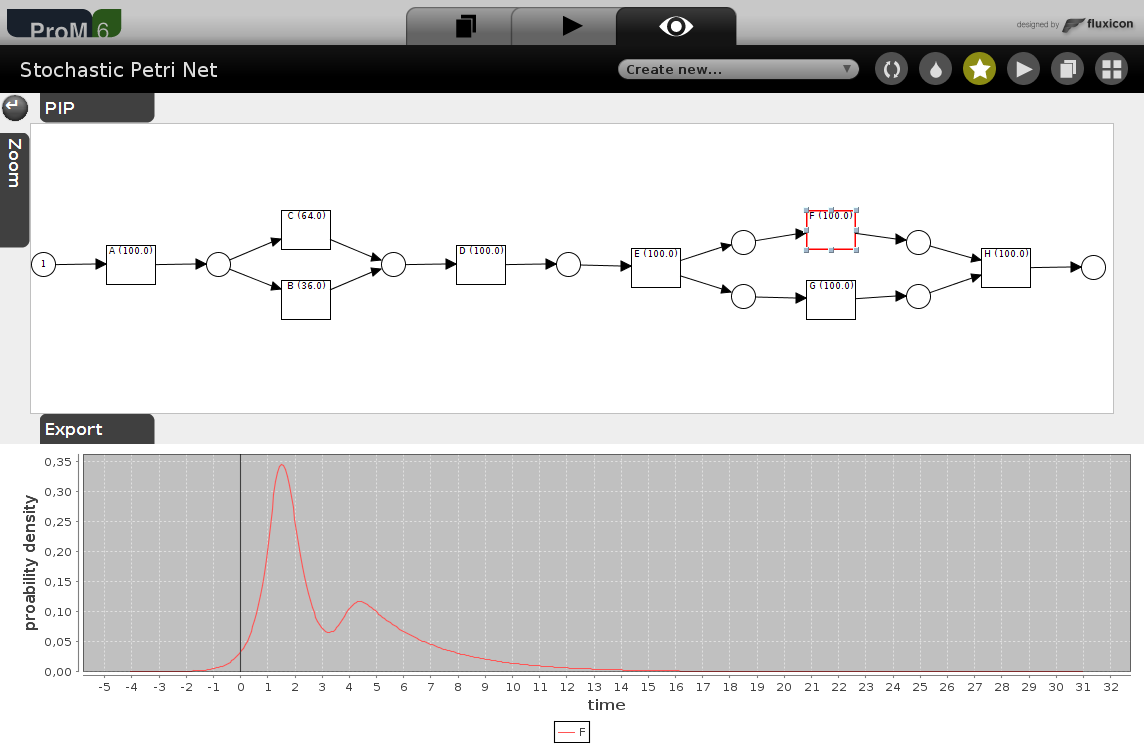
\includegraphics[width=0.95\textwidth]{visualize2_logspline.png}
\caption{Log-Spline distributions.}
\label{fig:log-spline_distributions}
\end{figure}
\section*{Hints \& Version changes}

\subsubsection{Useful Hints:}
\begin{itemize}
  \item Use the \emph{Configure Visibility of Transitions}-plugin to set transitions invisible, that do not appear in your log
  \item Always make sure, that your Petri nets are connected to a \textbf{final Marking}. Use the \emph{Create Final Marking Plugin} to achieve this.
  \item It is helpful to experiment with \textbf{simulated} Logs first, that \emph{fit} the Petri net. (Use CPN-Tools for example)
\end{itemize}

\subsubsection{Version changes}

\subsubsection{Initial version: 0.1}


\bibliographystyle{alpha}
\bibliography{refs}
\end{document}